\documentclass[../EBEXPaper2.tex]{subfiles}
\begin{document}
%------------------------------------------------- 
\subsubsection{Radiative Load}
\label{sec:optical_load}

\comred{sh didn't yet review this; need more conclusions on optical load}

The\footred{Potential data products to show: load vs time during the flight (saturation event), load as a function of the focal plane position, ... (FA)} power flowing from a bolometer to its thermal bath at temperature $T_0$ is described by 
\begin{equation}
P_{sat} (T_0) = P_{elec} (T_0) + P_{rad},
\label{eq:boloPowerFlow}
\end{equation}
where $P_{sat}$ is the power required to saturate the detector, $P_{elec}$ is the electrical power provided by the voltage bias, and $P_{rad}$ is the radiative power absorbed by the bolometer.
The saturation power depends on the physical properties of the bolometer and on $T_0$ as described in~\cite{irwin_book_2005}. 
We measure the detector saturation power in a dark test cryostat where the radiative power is negligible, as described in Section~\ref{sec:dark_measurements}. %by measuring the biasing electrical power while the detector is operated in a dark environment, where $P_{rad}$ is negligible.
The dark cryostats, however, typically have a bath temperature around 20-100~mK higher than the \ac{EBEX} bath temperature. 
Assuming the thermal conductivity follows a power law of power n, $\kappa = \kappa_{0} T^{n}$, 
%2.2, 1.9, and 2.1 for the 150, 250, and 410~GHz bands respectively \citep{hubmayr_thesis}, 
we calculate the power flow from the bolometer at temperature $T$ to the bath at temperature $T_0$ to be
\begin{equation}
%P = \frac{\int_{T_o}^T \kappa(T')dT'}{\int_0^l \frac{dx}{A(x)}} = \frac{A}{l} \frac{\kappa_0}{n+1}(T^{n+1} - T_{0}^{n+1}). %too much detail?
P = \frac{A}{l} \frac{\kappa_0}{n+1}(T^{n+1} - T_{0}^{n+1})
\end{equation}
where the bolometer's weak thermal link to the bath has a uniform cross section $A$ and length $l$.
The dark saturation powers are then adjusted to the \ac{EBEX} bath temperature via 
\begin{equation}
P_{sat}(T_0) = \frac{T^{n+1}-T_0^{n+1}}{T^{n+1}-T_{test}^{n+1}} P_{sat}(T_{test})
\end{equation}
where $T_0$ is the \ac{EBEX} bath temperature, $T$ is the bolometer temperature, and $T_{test}$ is the test cryostat bath temperature \citep{hubmayr_thesis}. 
We assume a thermal conductivity power of n=2 for all observation frequency bands.
We find the radiative power absorbed by the bolometer at float by differencing the saturation power measured dark, corrected to the \ac{EBEX} bath temperature, and the electrical power measured at float %comparing the saturation electric biasing power at float to the saturation power following 

\begin{equation}
P_{rad}^{float} = P_{sat}^{dark} - P_{elec}^{float}.
\label{eq:boloPopt}
\end{equation}

%\noindent after correcting for $T_0$.

Fig.~\ref{fig:dark_light_pv} shows an example of the radiative load measurement for bolometer 250-23-06-11, where the blue curve is the electrical power measured in a dark cryostat and the red curve is the electrical power measured at float.
%The electrical bias power is measured both in a dark environment and at float.
After adjusting the $P_{sat}^{dark}$ for bath temperature, we find the radiative power absorbed by this detector at float is XXX~pW. 
% tuning1, we saw 5.65pW, tuning2 we saw nan, tuning3 we saw 6.50
%\comred{would it be better to show a bolo tested at McGill since bath temperature closer to ebex? do we want to show this at all? we only adjust psat for bath temperature, not the whole curve. is it misleading to show the two curves?}
Fig.~\ref{fig:radiative_load_histograms} shows the distribution of the radiative load measured by all detectors for the first bolometer tuning of the \ac{EBEX2013} flight.
We measure an average load of 3.6, 5.2, and 4.9~pW for the 150, 250, and 410~GHz detectors, respectively.
Assuming the receiver efficiency is correct, the radiative loads measured for the 250 and 410~GHz detectors are compatible with the expected loads if the detector absorption efficiencies are 70\% and 40\%, respectively.
For the 150~GHz detectors, assuming a detector absorption efficiency of 80\% leads to an unexpected excess load of 1.7~pW as shown in~\cite{MacDermid_thesis}.
The absorption efficiency is further discussed in Section~\ref{sec:optical_efficiency}.
The excess loading in the 150~GHz band is thought to be due to optics spillover.
%\comred{Don't we also need to mention something about the assumptions we are making about the absorption/transmission/emission of everything upstream of the detectors??}

%\begin{figure}[htbp]
%\begin{center}
%\epsscale{1.0}
%\plottwo{images/detectors_and_readout/PV_250-23-09-07.png}{images/detectors_and_readout/load_tuning1.png}
%\caption{Right : the power as a function of the voltage bias as detector 250-23-09-07 is dropped in its superconducting transition in a dark environment (red) and at float (blue).
%\comgreen{The red curve does not match the dark power in the leap/resources.  Get a better looking bolo.}
%Left : the distribution of measured optical load at float (blue) per frequency band.
%The red line shows the expected load assuming 80, 70 and 40\% bolometer absorption efficiency.
%The green line is a gaussian fit with its parameter shown in the legend.
%\comred{Need to explain this distribution. JH}}
%\label{fig:boloPvCurve}
%\end{center}
%\end{figure}

%\begin{figure}[ht!]
%\begin{center}
%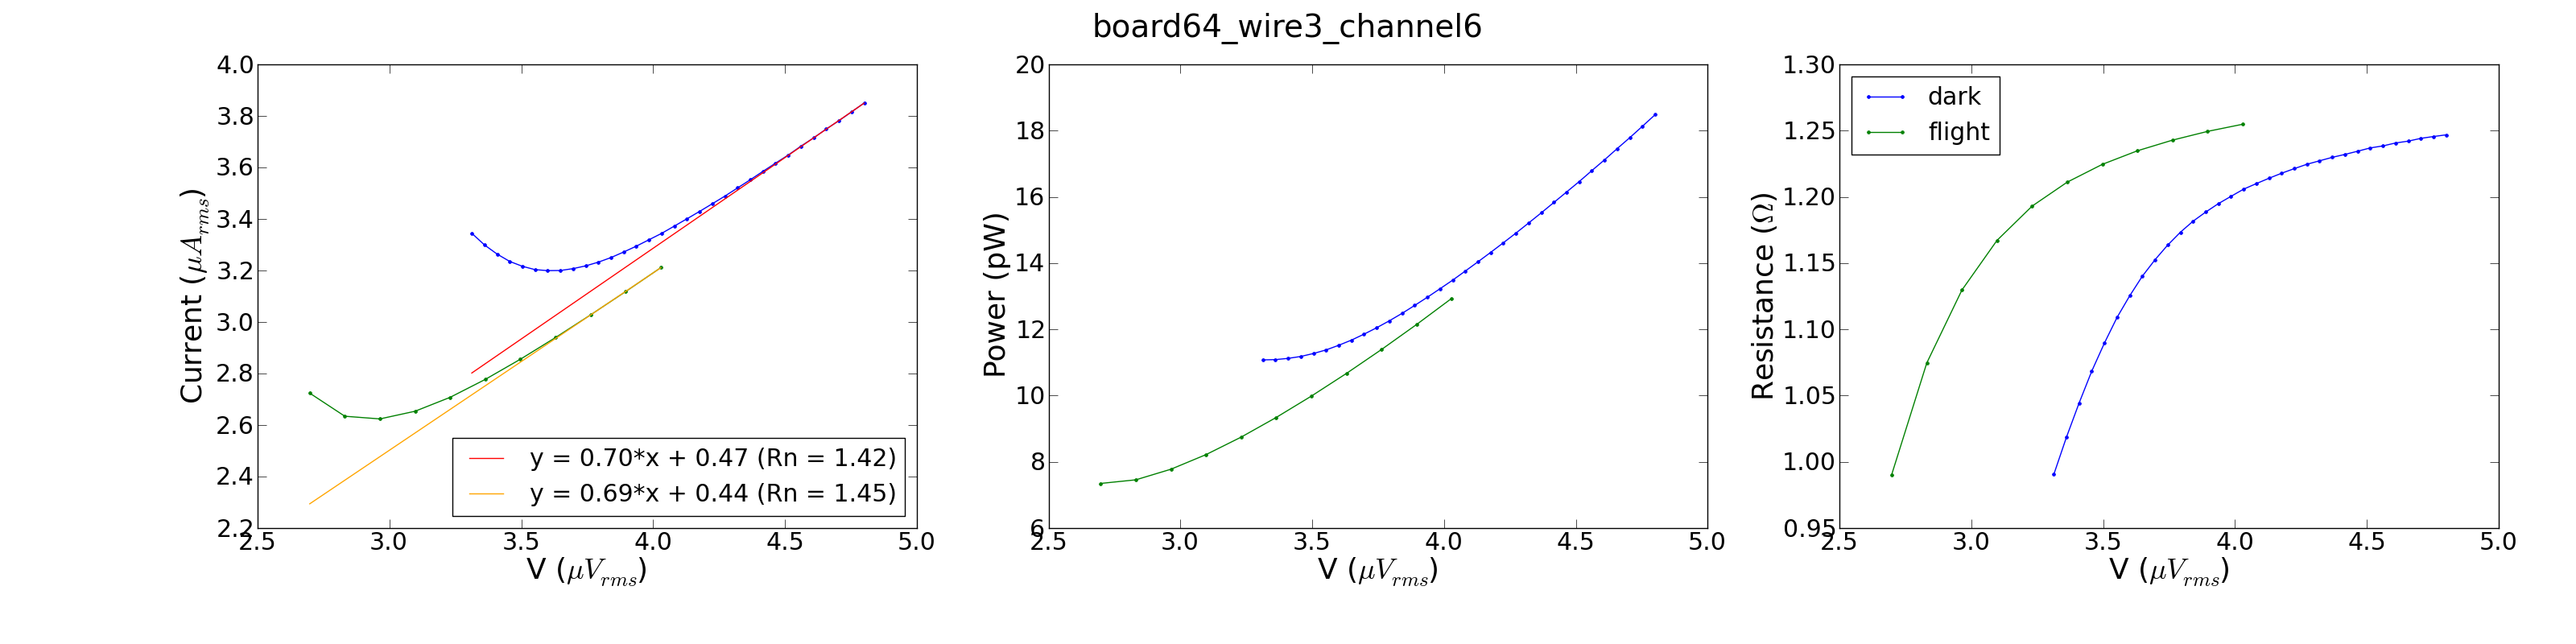
\includegraphics[height=1.7in]{images/board64_wire3_channel6_iv_curve}
%\caption{{\it Left:} Current through bolometer versus voltage bias. {\it Middle:} Electrical power dissipated in bolometer versus voltage bias. {\it Right:} Resistance of bolometer versus voltage bias.} \comred{Dark/light iv plots: this bolo tested in ETC, use McGill instead since bath temperature more similar? or just ignore subtlety that they're at different temperatures, so comparing on the same plot is slightly misleading and can't scale whole curve, but rather just last point? REMOVE title? REMOVE fits to iv? left-most/bottom-most axis numbers overlap. Legend in each plot with dark/light labels?}
%\label{fig: iv dark and light}
%\end{center}
%\end{figure}

\begin{figure}[htbp]
\begin{center}
\epsscale{1.0}
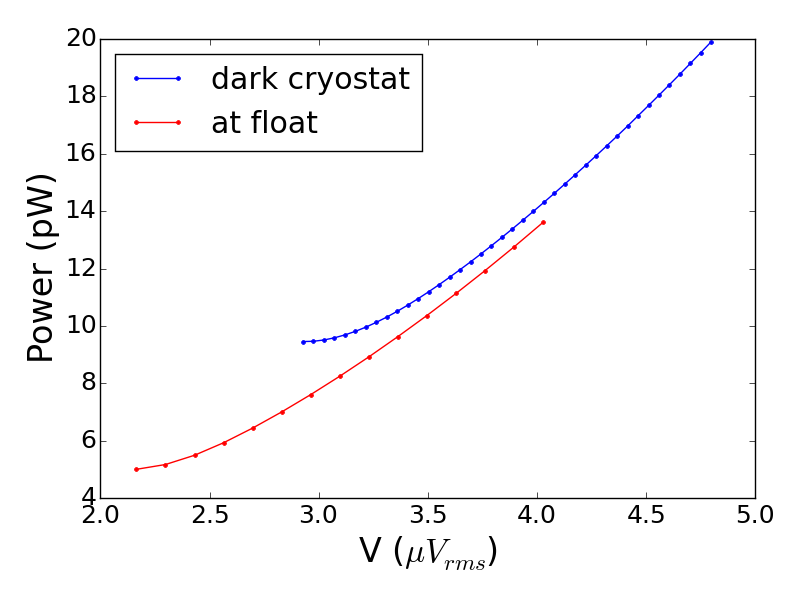
\includegraphics[height=1.7in]{images/board64_wire2_ch09_250-23-06-11_pv_curve}
\caption{The electrical power dissipated in the \ac{TES} as a function of the voltage bias for detector 250-23-06-11. As the voltage bias is decreased, the \ac{TES} temperature decreases. Once the \ac{TES} reaches its critical transition temperature, negative electrothermal feedback keeps the power dissipated constant. The blue curve is performed in a dark test cryostat at a bath temperature of $\sim$320~mK, and the red curve is performed in \ac{EBEX} at float with a bath temperature of $\sim$225~mK. The difference between the electrical power measured dark, corrected to the \ac{EBEX} bath temperature, and the electrical power measured at float is the measured radiative load.}
\label{fig:dark_light_pv}
\end{center}
\end{figure}


\begin{figure}[ht!]
\begin{center}
\begin{tabular}{cc}
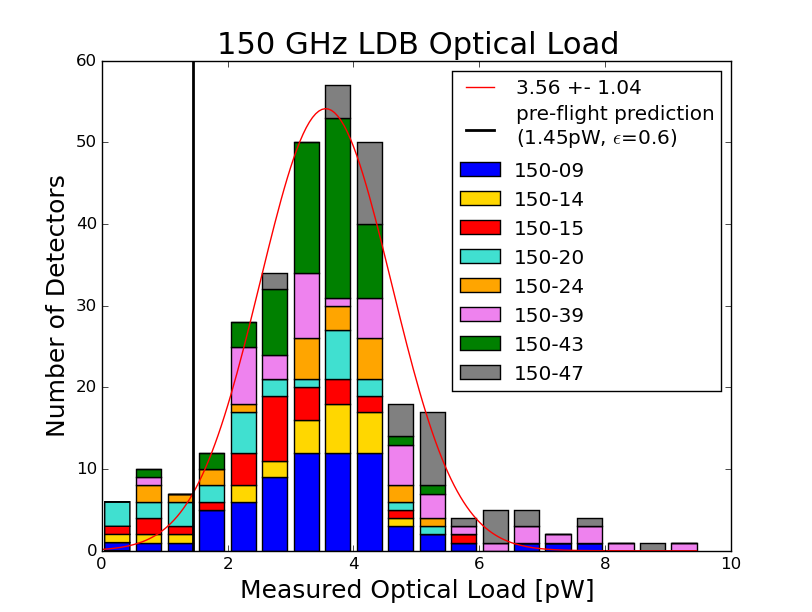
\includegraphics[width=0.33\columnwidth]{images/ldb_optical_load_150s}
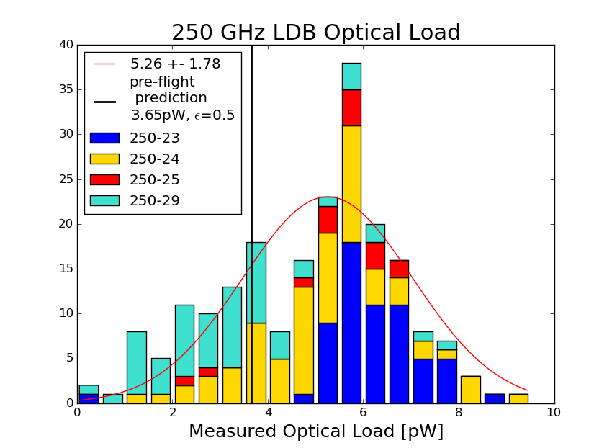
\includegraphics[width=0.33\columnwidth]{images/ldb_optical_load_250s}
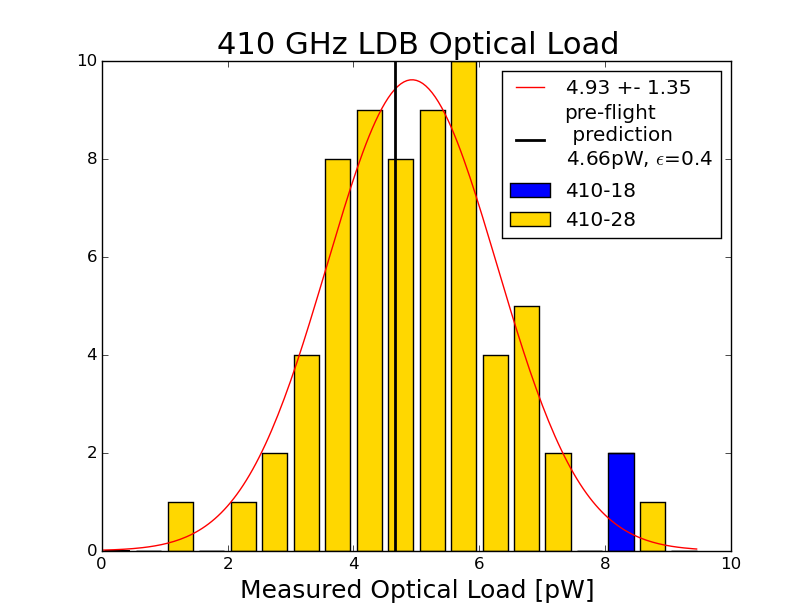
\includegraphics[width=0.33\columnwidth]{images/ldb_optical_load_410s}
\end{tabular}
\caption{Histograms of the measured radiative load from the beginning of flight for the 150~GHz band detectors ({\it left}), the 250~GHz band detectors ({\it middle}), and the 410~GHz band detectors ({\it right}). These are stacked histograms where each wafer is labelled with a different color. Each histogram is fit to a Gaussian distribution, red line. The average value and standard deviation from the fit are reported in the legend. The radiative load predicted pre-flight, assuming detector absorption efficiencies of 0.6, 0.5, and 0.4 for the 150, 250, and 410~GHz bands respectively, is indicated for each frequency band by a vertical black line.} \comred{clean up plots.} %some thoughts: 250~GHz plot needs to be same size as others, move legend to upper right to match? Y axis needs labelling. For 150~GHz, make pre-flight prediction two lines like others and eliminate parentheses. 410~GHz needs y axis label. All, put units on fit? Caption and text needs some words about $\epsilon$ and transmission/reflection/emission assumptions. Need larger axis numbers.}
\label{fig:radiative_load_histograms}
\end{center}
\end{figure}




%------------------------------------------------
%\include{DetectorReadoutBibliography}
\end{document}
